% Created 2020-06-03 Wed 22:09
% Intended LaTeX compiler: pdflatex
\documentclass[11pt]{article}
\usepackage[utf8]{inputenc}
\usepackage[T1]{fontenc}
\usepackage{graphicx}
\usepackage{grffile}
\usepackage{longtable}
\usepackage{wrapfig}
\usepackage{rotating}
\usepackage[normalem]{ulem}
\usepackage{amsmath}
\usepackage{textcomp}
\usepackage{amssymb}
\usepackage{capt-of}
\usepackage{hyperref}
\usepackage{todonotes}
\usepackage{apacite}
\usepackage{float}
\author{Njagi Mwaniki and you if you wanna ;)}
\date{\today}
\title{A Review of Genome Graph Tools}
\hypersetup{
 pdfauthor={Njagi Mwaniki and you if you wanna ;)},
 pdftitle={A Review of Genome Graph Tools},
 pdfkeywords={},
 pdfsubject={},
 pdfcreator={Emacs 26.3 (Org mode 9.2.4)}, 
 pdflang={English}}
\begin{document}

\maketitle
\begin{abstract}

\end{abstract}
\newpage
\tableofcontents
\listoffigures
\newpage
\section{Introduction}
\label{sec:org318c126}

There are four major overlapping steps that need to be carried out after DNA 
sequencing to get actionable results. 1) fragment assembly which involves 
recreating the original genetic sequence; 2) alignment, mapping, indexing and 
querying which are part of the assembly stage but can be done later to query the
relatedness of sequences; and 3) Visualization to see these changes.\cite{flicekSenseSequenceReads2009}
\todo{expand intro}

\section{Fragment Assembly}
\label{sec:org8cbfbb1}
The fragment assembly problem, reconstructing long contigs from reads
\cite{chikhiCompactingBruijnGraphs2016}, started with Sanger sequencing.
Like solving a puzzle of sequences the assembly problem can be framed as finding
a set of common super-strings from a set of substrings to which tools take 
either a Eulerian, connect the nodes, or a Hamiltonian, connect the edges, 
approach.

The first solution was SEQAID, short for \textbf{seq}uencing \textbf{aid},
\cite{peltolaSEQAIDDNASequence1984} which used the  Overlap Layout Consensus (OLC)
framework, an intuitionistic approach to the assembly problem that works in  
3 main steps: 1) Overlap: find all overlaps among the reads, 2) Layout: assemble
a graph of all the reads based on their overlaps, and 3) Consensus: infer the
consensus sequence.

What it does is find the overlaps between the given set of reads and then lays 
them out to form a DAG. The graph, however, has multiple paths that are the 
genome or superstring in question. Which is where the consensus comes in. 
It used … to infer the consensus.

\begin{figure}[H]
\centering
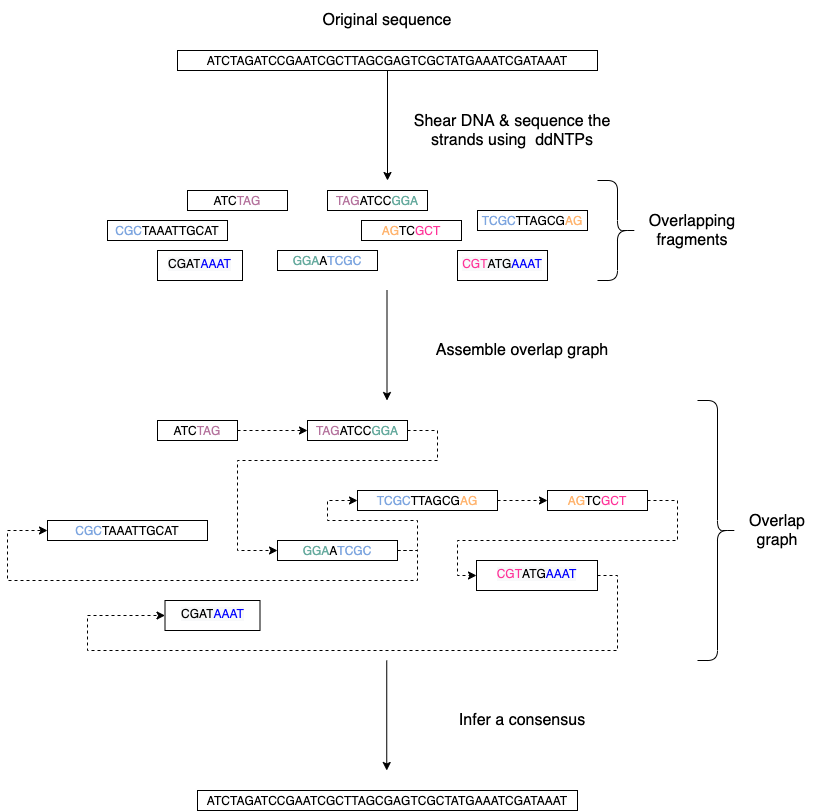
\includegraphics[width=0.7\textwidth]{assets/images/OLC framework.png}
\caption{OLC...}
\end{figure}

With the advent of Second Generation Sequencing (SGS) technologies 
Roche/454 (www.454.com), Illumina/solexa (www.illumina.com),
and AB/Solid (www.appliedbiosystems.com) there was a significant reduction in 
the cost per sequenced nucleotide \cite{liComparisonTwoMajor2012} leading to an 
explosion in the number of reads produced and thus making OLC unfeasible. 

OLC based methods were progressively replaced by de Bruijn Graph (DBG)
\cite{iduryNewAlgorithmDNA1995} based methods whose first tool was EULER
\cite{pevznerEulerianPathApproach2001}.

The DBG transforms the assembly problem into a computationally simpler problem.
While the OLC, through the reads graph, takes an non polynomial time Hamiltonian 
approach; the DBG, using the k-mer graph, goes about it using a much easier to
solve Eulerian approach which works in polynomial time.
\cite{liComparisonTwoMajor2012,pevznerEulerianPathApproach2001} 

The DBG is an anti-intuitionistic solution whose assembly quality improves with 
an increase in the read length <cn>. It works through 1) chop the reads into
much smaller k-mers, 2) Use all the k-mers to assemble a dBG, 3) Infer the 
genome sequence on the dBG. These tools made it possible to work with the 
increasing number of reads produced. 

\begin{figure}[H]
\centering
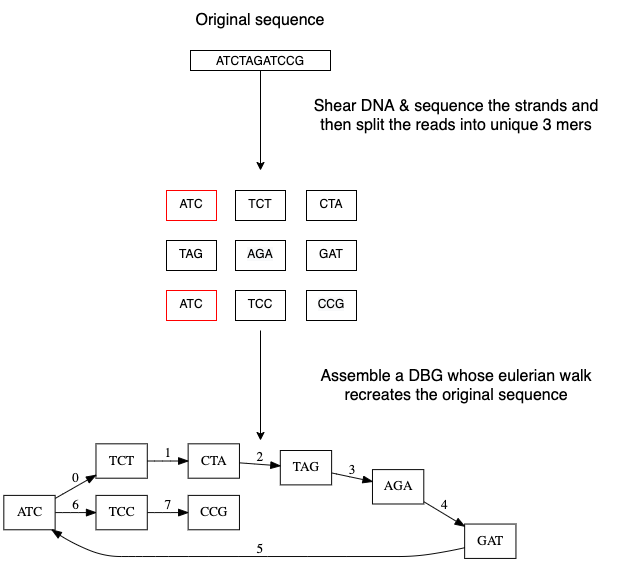
\includegraphics[width=0.7\textwidth]{assets/images/de Bruijn Graph.png}
\caption{DBG...}
\end{figure}

Lately, Single Molecule Sequencing (long read sequencing)  methods have 
reintroduced OLC for the assembly of long erroneous reads but DBG based methods 
are still used to correct long reads.
The unitig approach involves finding the maximal interval subgraphs in the
graph of all read overlaps.

The string graph \cite{myersFragmentAssemblyString2005} is a way to infer the 
genome from the read data without a need for k-mers as is with the de Bruijn 
graph.  It treats the genome as a sequence of repeats and then “encodes” each 
repeat as a node. Each unique (contiguous) sequence is a node. 
An Eulerian tour recreates the genome.

\begin{figure}[H]
\centering
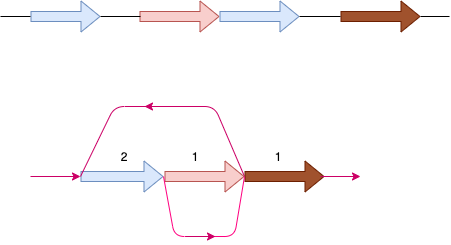
\includegraphics[width=0.7\textwidth]{assets/images/String Graph.png}
\caption{String Graph...}
\end{figure}\label{string graph}

\section{Alignment and mapping}
\label{sec:org17542ca}
Alignment involves computing the amount of similarity between two strings also 
known as the edit distance problem.
The solution to the edit distance problem by
\cite{levenshteinBinaryCodesCapable1966a} paved the way for solving the alignment
problem.

The first solution was global alignment
\cite{needlemanGeneralMethodApplicable1970} in which a sequence query is aligned
to the other (reference) in its entirety. It took a dynamic programming approach
which worked in square time (had a complexity of O(n\textsuperscript{2}); it was followed by 
semi-global alignment \cite{sellersTheoryComputationEvolutionary1980}
where one sequence (query) is entirely
aligned to a substring of the other (reference); then local alignment
\cite{smithIdentificationCommonMolecular1981}, where the alignment can be between 
any substrings of the two sequences.

In practice when given a set of reads, a complement of each read is generated to 
be searched against because of the direction of sequencing or inversions.
A match can either be exact, matching the pattern exactly, or fuzzy, where a 
section or all of the string matches the pattern approximately, with minimum 
edit distance.

With graphs, reads are mapped to paths in the graph instead of linear sequences.
Alignment problems grow with the input size
\cite{durbinEfficientHaplotypeMatching2014} making it hard to align sequences to
graphs  because of the increased amount of data involved
The complexity of an alignment problem is a function of the
number of  vertices |V| and edges |E| <cn>.  In some way you can think of it 
as mapping to multiple linear sequences that may or may not loop.

\section{Indexing}
\label{sec:orgce10310}
Indexing is a solution to the problem of search given limited computing
resources. An index is useful to speed up alignment and make it pragmatic within
the given time and memory requirements. 
It involves reducing the search space so as to reduce the time taken and memory
consumed when performing a search.
In linear references commonly used indexing approaches are the FM index 
todo\{list tools\} whose complexity is O(NM) where there are N variable sites and 
M sequences \cite{durbinEfficientHaplotypeMatching2014}.
As in alignment, the problem grows even larger with the proliferation of paths 
in graphs. For graphs, indices like the FM-index backed by the BWT fail to hold<cn> 
and there’s the need for improvements such as that seen in gBWT used in seqwish 
allowing it to be orders of magnitude faster than VG.

An index can either be static or dynamic. A static index is serialized and saved
to disk while a dynamic index is created at runtime and held in memory. Dynamic
indices are good with small datasets that change rapidly such as in the
construction of a DBG making it suitable for fragment assembly. Static indices 
are suited for larger datasets that we want to go back to such as a reference
genome graph.

Below are some of the approaches taken to solve the problem of indexing
\subsection{Burrows-Wheeler Transform}
\label{sec:org2e1aa8c}
The Burrows-Wheeler Transform (BWT) was introduced by
\cite{burrowsBlocksortingLosslessData1994} for string data 
compression and to this day forms the basis of the bzip compression algorithm.

It works as a preliminary step in the building of indices and also the 
compression of \todo{expound}


\subsection{Suffix Array}
\label{sec:orgf9facc7}
Suffix arrays were introduced by \cite{manberSuffixArraysNew1990} are arrays of
the positions of all the sorted suffixes of a string. 
A suffix array is a simple, space efficient 
(stores n integers where n is the length of the string) alternative to the
suffix tree <citation needed> whose space requirements are\ldots{}
based on BWT have been used for fast search algorithms

Improvement to the suffix array: \cite{liMinimapMiniasmFast2016}
gave the first in-place O(n) time suffix array construction algorithm that is 
optimal both in time and space, where in-place means that the algorithm only
needs O(1) additional space beyond the input string and the output suffix
array.

Tools using the suffix array include Bowtie
\cite{langmeadUltrafastMemoryefficientAlignment2009}, BWA
\cite{liFastAccurateShort2009}, 
and SOAP2 \cite{liSOAP2ImprovedUltrafast2009}.

\subsection{FM Index}
\label{sec:org886eca9}
Short for Full-text index in Minute space; the FM-index created
by \cite{ferraginaOpportunisticDataStructures2000} is a full text substring index
based on the BWT. It allows compression of the input text while permitting fast
substring queries. It can be used to efficiently find the number of occurrences
of a pattern within the compressed text, as well as locate the position of each
occurrence.

\subsection{Positional Burrows-Wheeler Transform}
\label{sec:org43011ae}
Introduced by \cite{durbinEfficientHaplotypeMatching2014} Positional Burrows 
Wheeler Transform is an algorithm with complexity O(NM) where M sequences and
N bi-allelic sites.
It derives a representation of the data based on a positional prefix array; an
array that holds positions of a given array/set of haplotypes in a larger 
haplotype array. This prefix array orders them in reverse (ascending) order of
their prefixes allowing similar sequences to cluster together.

<Add PBWT table and graphic>

\subsection{GBWT/gPBWT}
\label{sec:org3f8856a}
First described \cite{novakGraphExtensionPositional2017} but used in a tool
\cite{sirenHaplotypeawareGraphIndexes2020} it’s a compressible representation of 
a set of haplotypes held in the graph. This allows for efficient match queries 
in sections of the haplotypes (local alignment). Because of the previously
mentioned nature of the positional suffix array to bring together (fairly) 
similar haplotypes. 
GBWT lets us have an efficient way of counting the number of haplotypes 
containing a given sequence.

\subsection{Bloom filters}
\label{sec:orgb74acef}
The bloom filter is a probabilistic data structure that can give false positive
but never a false negative.  It works by hashing data and stores the hash in an
array\ldots{}
It is suited for the fragment assembly using DBGs because of its constant time
access \cite{chikhiSpaceefficientExactBruijn2013}. It however suffers from poor
data localization \todo{expound} which led to the use of Blocked Bloom Filters (BBF) 
\cite{putzeCacheHashSpaceefficient2010} used in
Bifrost \cite{holleyBifrostHighlyParallel2019}.

\subsection{Minimizers}
\label{sec:orgf5af696}
The work of a minimizer is to reduce the search space. It does this by generating
kmers from a read and sorting them alphabetically. The k-mer at the top is the
minimizer for that read\ldots{} then binning the result. When a query is made it’s
prefix is checked against the bin and the rest of the data ignored
<is this even accurate?>
We can get a minimizer by BBF blocked bloom filter Minimizers
\cite{grabowskiDiskbasedCompressionData2015,robertsReducingStorageRequirements2004}

\subsection{Hash tables}
\label{sec:org3e51007}
Hash tables involve breaking down the reads into k-mers and storing the kmers
into hash tables that point to the original data. When queries are made they’re 
similarly broken down into k-mers of the expected size<citation needed>.
Hash based methods when well tuned can be faster than suffix array based 
methods, because the basic operations are simpler, but they typically require
greater memory, particularly in cases where the suffix representation can be
compressed as it can be here (Durbin 2014).
Many times tools take a hybrid approach; incorporating different aspects of
different indexing schemes such as in Minimap
\cite{liDesignConstructionReference2020}. \todo{ensure this citation checks out}
\section{Genome Graph Tools}
\label{sec:orgc7cb93d}
The Berkeley Open Assembler \cite{myersFragmentAssemblyString2005} uses the 
string graph \ref{string graph}, a way to infer the genome from the read data 
without a need for k-mers, and borrows from the unitig algorithm.
It treats the genome as a sequence of repeats and then “encodes” each repeat as 
a node. Each unique (contiguous) sequence is a node. An Eularian tour recreates
the genome.
Though the original DBG approach does much better than OLC it still has a high 
memory footprint<citation needed>.

Minia \cite{chikhiSpaceefficientExactBruijn2013} proposed the use (encoding) of a 
DBG as a bloom filter (BF) instead of storing the graph in a “traditional” set
series of nodes and edges stored in <mention tool>. 
By design, a bloom filter can give a false positive result but never a false
negative therefore the name probabilistic de Bruijn graph. It is obtained by 
inserting all the nodes of a de Bruijn graph (i.e all k-mers) in a BF. 
A BF has a search/access time of O(1). They then had an additional structure to 
remove critical false positives. It showed that the graph can be encoded with 
as little as 4 bits per node.
Drawbacks include 1) The Bloom filter introduces false nodes and false
branching, 2) The global structure of the graph is approximately preserved up to
a certain false positive rate.

Bcalm2 \cite{chikhiCompactingBruijnGraphs2016} tried to improve this by use of 
compacted DBG (cdBG). It allowed the problem to be doable on a PC.

\todo{<add compaction diagram>}

The use of the de Bruijn graph in fragment assembly consists of a multi-step 
pipeline.
The most data intensive steps are usually the first three: 
nodes enumeration/k-mer counting: the set of distinct k-mers is extracted from 
the reads 
Compaction: all unitigs (paths with all but the first vertex having in-degree 1
and all but the last vertex having out-degree 1) are compacted into a single 
vertex
graph cleaning: artifacts due to sequencing errors and poly- morphism are 
removed from the graph

<image explaining compaction>

Minimap \cite{liMinimapMiniasmFast2016} introduced two tools minimap, a raw read 
overlapper, and miniasm \cite{liMinimapMiniasmFast2016}, an assembler. 
Minimap uses minimizer sketches, stores k-mers in a hash table, uses sorting 
extensively.
SPAdes  also a toolkit does…

\newpage
Variation graphs embed the paths in the graph. 
These paths can be used to represent haplotypes. vg, HashGraph,
odgi and PackedGraph are dynamic (allow for updates to the graph while xg isn’t).

\begin{center}
\begin{tabular}{llllllll}
Individual 1 & A & C & T & G & A & A & T\\
Individual 2 & A & C & T & T & - & - & T\\
Individual 3 & A & C & T & T & A & A & T\\
\hline
Consensus & A & C & T & T & A & A & T\\
\end{tabular}
\end{center}


\begin{figure}[H]
\centering
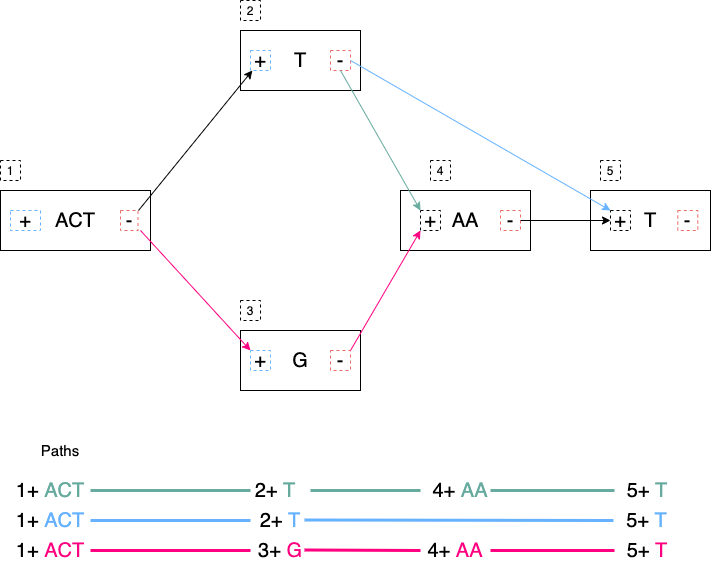
\includegraphics[width=0.7\textwidth]{assets/images/Variation Graph-Page-1.png}
\caption{no structural variation}\label{no struct}
\end{figure}

\newpage
In case of addition of individual 4 containing an inversion at node 2,3 and 4

\begin{center}
\begin{tabular}{llllllll}
Individual 1 & A & C & T & G & A & A & T\\
Individual 2 & A & C & T & T & - & - & T\\
Individual 3 & A & C & T & T & A & A & T\\
Individual 4 & A & C & A & A & T & T & T\\
\hline
Consensus & A & C & T & T & A & A & T\\
\end{tabular}
\end{center}

\begin{figure}[H]
\centering
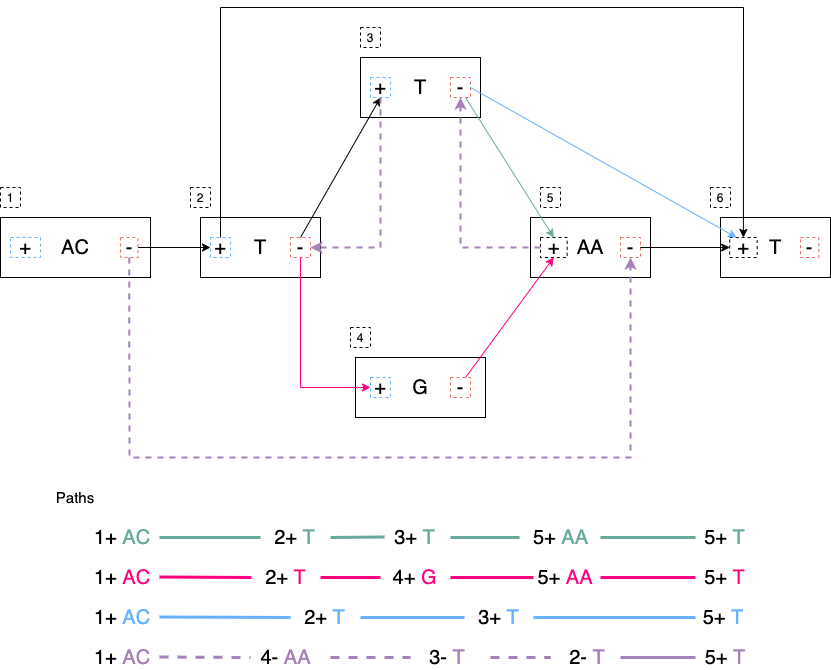
\includegraphics[width=0.7\textwidth]{assets/images/Variation Graph-Page-2.png} 
\caption{contains struct variation}\label{contains struct}
\end{figure}

vg \cite{garrisonVariationGraphToolkit2018} used the protobuf library as the 
graph implementation but was refactored to use the HandleGraph API as of 1.22.0.
It is an end to end pangenome graph solution for de novo and incremental graph
building but has large memory requirements when it comes to indexing. 
How it deals with cycles in the graph: unrolls the graph with cycles. 
The graph holds nodes in a vector. It uses hash tables to map between nodes and 
ids in a vector that holds the nodes. Paths are stored in a set of linked lists. 
A hash table maps between nodes and paths. Suffered from a problem of data
duplication.
Queries involve hash table lookups.
xg \cite{garrisonGraphicalPangenomics2019} a memory-efficient succinct 
representation of the graph (compared to vg). 
It being static and having indexing of the paths using positional indices, GBWT,
allows it to have fast queries making it good at  read mapping and variant 
calling.

Bluntification \cite{gargGraphbasedApproachDiploid2018} removing all overlaps 
between nodes seqwish (\url{https://github.com/ekg/seqwish}) transforms a set of 
sequences and alignments (in GFA) into its equivalent variation graph.
The large memory requirements of vg are solved through the use of gBWT backed
by a Generalized Compressed Suffix Array. It’s still a static index odgi
(libhandlegraph paper) Optimized Dynamic Graph Interface, uses a dynamic index
and uses an in memory variation graph to perform sorting, pruning, 
transformation, and visualization.

HashGraph (libhandlegraph paper) has speed as its primary goal. 
Represents a graph as a high performance hash table. 
Paths are embedded as double linked lists. Edges are in vectors attached to 
each node they connect. Use an adjacency list which is appropriate for sparse graphs. 
Appropriate for small graphs <such as viruses> because it trades memory for time.
Odgi (libhandlegraph paper) is based on a node centric encoding of the graph that 
is designed to improve cache coherency when traversing or modifying the graph. 
It tries to be a pragmatic tool that achieves balance between memory usage and
performance. Each nodes seq and edges are encoded in a byte array using a 
variable length integer, edges are described in terms of the relative offset of 
a node in a sorted graph. PackedGraph (libhandlegraph paper) is designed to have
a low memory footprint. 
It does this by encoding the graph mainly using linked lists.
Baum \cite{wangBAUMImprovingGenome2018} By Adaptive Unique Mapping (BAUM) improved
on the OLC framework  to improve genome assembly based on SGS
paired-end/mate-pair libraries.

BAUM has two modules: construction of the genome unique regions that are taken
as the initial contigs iterative assembly, in which scaffolds are built, and 
contigs are extended and merged, aiming to reconstruct the repetitive regions 
along the iterations.
In this scheme, the repetitive regions are separated by the unique regions
Bifrost \cite{holleyBifrostHighlyParallel2019} improved on the cdBG by adding 
colours and takes advantage of concurrency (parallell) to the nodes to keep 
track of the source of each vertex.
Size of colours can grow beyond that of the nodes In the output 
it stores these colours in a different on a different .bfg\textsubscript{colors} file.
K-mers contained in the unitigs are mapped to their colors representing the
input sources (color is represented by an integer from 1 to |C| where C is the
number of colors. Colors are stored in a separate array of color containers,
each color container is indexed by MPHF (Minimal Perfect Hash Function) library
BBHash \cite{limassetFastScalableMinimal2017}.
BF has poor data localization because one element is scattered all over which 
leads to CPU cache misses when inserting and querying are addressed here 
(Putze et al., n.d.) for this they used (BBF) blocked bloom filter 
Minimizers \cite{robertsReducingStorageRequirements2004,grabowskiDiskbasedCompressionData2015}.
BBF works by building an approximation of the dBG using BBFs to filter our
seq errors. 
BBF containing k-mers is used to build the cdBG.

GraphAlighner \cite{rautiainenBitparallelSequencetographAlignment2019} is a tool 
for aligning long error prone reads to genome graphs. It performs base alignment.
It uses (generalizes two linear sequence-to-sequence algorithms to graphs) two 
strategies: the Shift-And algorithm for exact matching (exact match of a
substring to a string) and Myer’s bit-vector algorithm for semi-global alignment
Aligns sequences to graphs while exploiting bit parallelism. Makes use of
Nondeterministic Finite Automaton (NFA). Store an NFA state bitvector for
each node and update until no more change is necessary
Myer’s bit-vector algorithm studies the semi-global sequence-to-graph alignment 
problem. It seeks to find a path in a directed, node-labelled graph that has the
minimum edit distance to the query sequence. Myers’ bit-vector alignment 
algorithm (Myers, 1999) to graphs, which proceeds along the same lines as the
Shift-And algorithm, but requires some further algorithmic insights to handle 
nodes with an in-degree greater than one. Bitvector algo complexity grows 
approximately linearly with the number of vertices in the graph. The bitvector 
it uses is the size of the pattern we are searching for. Semi-global alignment 
is solved through generalizing DP edit distance problem for graphs. Semi-global 
alignment is used to align a shorter seq against a longer one, reference.
Shift-And algorithms (Baeza-Yates and Gonnet, 1992; Domolki, 1964, 1968) 
performs exact string matching to graphs. 
Their aim is to find a path in a directed, node-labeled graph that has a minimum
edit distance \cite{levenshteinBinaryCodesCapable1966a} to the query sequence. 
Shift-And algo finds exact matches between a pattern string and a text string by
simulating a nondeterministic finite automaton (NFA) that matches the pattern 
and then feeding the text to it.
Keep shifting the bit-vector by one and bitwise AND-ing the state. 
Somewhat analogous to exact matching using a window of the size of the pattern.
It can handle DAGs and  graphs that may contain cycles. For DAGs, process the 
nodes in topological order (topological sort). For cyclic graphs no sorting.

Minigraph \cite{liDesignConstructionReference2020}, for incrementally constructing 
reference variation graphs,
is a sequence to graph mapper that incrementally constructs a pangenome graph.
A graph-based data model and associated formats to represent multiple genomes 
while preserving the coordinate of the linear reference genome. 
A straightforward way to represent a pangenome store unaligned genomes in a
full-text index that compresses redundancies in sequences identical between 
individuals (Boucher et al., 2019; Liu, Zhu, et al., 2016; Mäkinen et al., 2010) 		
The other class of methods encodes multiple genomes into a sequence graph, 
usually by collapsing identical or similar sequences between genomes onto a 
single representative sequence. The results in a pangenome graph.

GraphAlighner performs base alignment but minigraph does not. Minigraph is
faster than GraphAligner and uses less memory. Minigraph is more accurate than
GraphAligner. This is counter-intuitive given that GraphAligner does base alignment. 
Close inspection reveals that most mismapped reads by minigraph are mapped to the
correct genomic loci but wrong graph paths. On the contrary, most mismapped
reads by GraphAligner are mapped to wrong genomic loci. Vg didn’t work with 
their PacBio data. vg allows different regions in one chromosome collapsed to one
segment. We call such a graph a collapsed graph. rGFA cannot encode a collapsed
graph.

vg-flow \cite{baaijensStrainawareAssemblyGenomes2020} attempts to reconstruct all 
individual haplotypes from a mixed sample at the strain level and to provide
abundance estimates for the strains. It does this by\ldots{}

\section{Interfaces and APIs}
\label{sec:org35c7c7b}
The field of genome graphs is growing quickly as evidenced by the ever-growing
number of tools creating the need for a common way for these tools interact with
the data they operate on.

One such solution is libhandlegraph, a declarative approach towards graphs that
defines an interface between which tools interact with the data below. 
The idea is to treat the graph as a larger structure to which we have pointers,
called handles (similar to  Unix file handles), through which we manipulate the
graph. 

\begin{figure}[h]
\centering
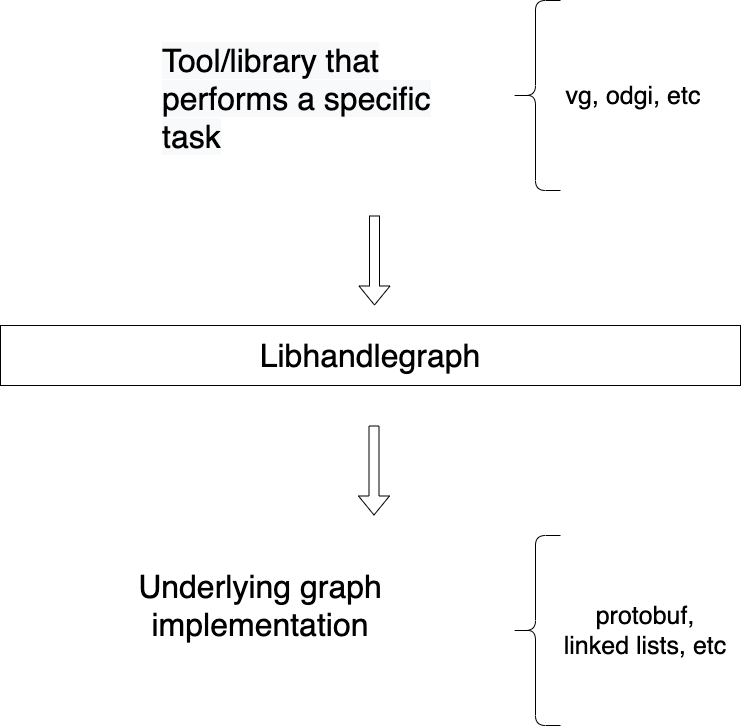
\includegraphics[width=0.7\textwidth]{assets/images/libhandlegraph.png}
\caption{libhandlegraph...}
\end{figure}

libhandlegraph is primarily used in vg as an abstraction layer over different
backing graph implementations.
It defines a common set of attributes and operations through which we can
manipulate the graph. We can then use the libhandlegraph API as a layer between
an underlying graph implementation and genome graph manipulation tools we plan 
on building.

libhandlegraph has python bindings and is now being ported to Rust. In C++ and 
Python, it uses the class abstraction while in Rust the trait abstraction.

libbdsg (Optimized bidirected sequence graph implementations for graph genomics)
is a C++ library that provides high performance implementations of sequence 
graphs for graph-based pangenomics applications. Tools built on top of this are
PackedGraph (low memory) and HashGraph (high-performance hash tables).
vg is now using libhandlegraph through libbdsg (libhandlegraph paper).

\section{Plaintext graphical representations}
\label{sec:org811773d}
In the early 2000s assembly software was dominated by a few end to end assembly
software such as SPAdes, ALLPATHS, ABySS, and SOAPdenovo
\url{https://pmelsted.wordpress.com/2014/07/17/dear-assemblers-we-need-to-talk-together/}.
These end to end tools made it hard to tweak parts of the assembly process which
led to calls (such as \href{https://github.com/pjotrp/bioinformatics\#the-small-tools-manifesto-for-bioinformatics}{THE SMALL TOOLS MANIFESTO FOR BIOINFORMATICS}) for small
tools that perform bits of the assembly while using plaintext files as APIs.

An early attempt was FASTG,  an extension to FASTA, which is based on a directed
graph (digraph) and was originally meant to represent variability in the final
output of the assembly process.
It encodes the sequences on arcs/edges and refers to the connection
between sequences as vertices.

Like FASTA, each record contains a header line which follows the pattern
a greater than sign, the edge, the neighbors of the edge and the edge properties.
\(>Edge:Neighbours:Properties;\) where: Edge is the name given to this 
edge/sequence, Neighbors is a list of edges or their reverse complements that
follow this edge or the reverse complement of this edge
(indicated by a preceding\textasciitilde{}), and Properties is a list of optional properties 
associated with this edge. To facilitate
inversions, the format allows for adjacencies between forward and reverse
complement. Reverse complements are indicated by a prime symbol 30\textprime.

\begin{verbatim}
>x:y;
ACGTGAGAT
\end{verbatim}
An example of a FASTG fragment where x represents
a DNA sequence and an edge in the graph. The edge is in turn followed by edge y. 
There exists an adjacency from edge x to edge y.

GFA \cite{liMinimapMiniasmFast2016} comes in two versions:
GFA1 (\url{https://gfa-spec.github.io/GFA-spec/GFA1.html}) and
GFA2 (\url{https://gfa-spec.github.io/GFA-spec/GFA2.html}) with GFA2 being a superset
of GFA1. 
Unlike FASTG, GFA is a total deviation from the FASTA format aimed specifically 
at plaintext representation of genome graphs and able to represent a graph at 
all stages of the assembly <cn> as well as varying topologies (can encode bubbles).
Unlike FASTG, it encodes the sequences on the nodes, which it names segments and
has edges as the connections between segments. 
Each line must begin with either H (header), S (Segment), F (Fragment), E (Edge),
G (Gap) and G or U (Group) and each token is separated from the next by a tab
(is tab delimited). 
It can encode extra detail through fragments which are used to specify a
collection of external sequences or edges which may contain a Dazzler-trace or
a CIGAR string to describe the alignment of the edge.

rGFA \cite{liDesignConstructionReference2020} is GFA extended for reference 
(pan)genomes. It is an extension
to GFA with 3 additional tags that indicate the origin of the segment to
provide a unique stable coordinate system as an extension to the linear 
reference coordinate. Each segment is associated with one origin which forbids
collapsing of different nodes from one region as would be with a cDBG  in the
graph by design. rGFA disallows overlaps between edges and forbids multiple
edges (more than one edge between the same pair of vertices). 
To make use of the reference pangenome graphs 
GAF \cite{liDesignConstructionReference2020} is a text format 
for sequence to graph alignment.
It’s an extension of PAF \cite{liMinimapMiniasmFast2016}. 
It is tab delimited like GFA. \todo{describe the grammar}

\section{Genome graphs as databases (logic programming)}
\label{sec:orgf65da1b}
We can also treat the variation graph as a graph database. For this, SpOdgi 
\todo{citation needed} transforms any odgi genome variation graph file into a
SPARQL capable database.

\section{Visualization}
\label{sec:orge12209e}
Visualization tools are a core tenet of bioinformatics and science in general.
They help us understand our assemblies and communicate the results with others. 
Different tools exist depending on the level of resolution needed and 
the size of the graph. 

GraphViz \cite{northOnlineHierarchicalGraph2002,ellsonGraphvizDynagraphStatic2004}
is a collection of different graph visualization tools \todo{expound}

Bandage \cite{wickBandageInteractiveVisualization2015}, originally developed for 
assembly graph visualization, is a standalone application written for
visualizing assembly graphs.
It allows the visualization of several contigs which they themselves may have
various paths within them.
It uses a force-directed layout via, strength is aesthetic appeal and clearly
communicates components but annotation and navigation aren’t possible.
The major issue is the runtime scalability; force-directed layout has quadratic 
or even cubic costs with respect to graph size \todo{cite pantograph docs}.
The Open Graph Drawing Framework library (\url{http://www.ogdf.net/}) is used to
perform the graph layout using the fast multipole multilevel layout algorithm, 
which scales well for very large graphs (Hachul and Ju ̈ nger, 2007).
It reads a graph in a variety of formats: LastGraph (Velvet), FASTG (SPAdes), 
Trinity.fasta, ASQG and GFA and allows the export of a visualization graph
either entirely or a section of it (\url{https://rrwick.github.io/Bandage/}).

MoMI-G \cite{yokoyamaMoMIGModularMultiscale2019}
(MOdular Multi-scale Integrated Genome graph browser) 
is a web based genome browser built for the visualization of structural 
variants (SVs) in a variation graph and has a chromosome centric view making
it best for prokaryotic, <containing chromosomes> genomes. 
It works through a server client web architencture where the client (browser)
makes requests to a backend server that one can set up locally using docker.
It takes as input: a succinct representation of a variation graph in XG format,
read alignment (optional), and annotations (optional).

Sequence tube maps \cite{beyerSequenceTubeMaps2019} is a javascript module that
can be accessed within MoMi-G for the visualization of variation graphs or one
can  build their own custom API to generate the data whose aim is to represent
both structural variation and sequence alignments.
Tube maps were initially built to represent public transportation networks,
London’s iconic Tube Map, \cite{cartwrightamBeckRepresentationLondon2012} which 
themselves were inspired by circuit diagrams.

For visualizing large graphs which contain paths, assembly graphs which are de 
Bruijn graphs don’t contain paths, it’s recommended to use a pipeline such as …
These break a large graph into “chunks” that can be visualized bit by bit. 
Pantograph (2020) is another web based variation graph browser. 
It renders the genome graph in a matrix. It reads a variation graph in JSON from
odgi bin.

\todo{Add image of our Household 20 dataset in pantograph}


\bibliographystyle{apacite}
\bibliography{library}
\end{document}
